\documentclass[12pt]{article}

\usepackage{amsmath}
\usepackage{multirow}
\usepackage{microtype}
\usepackage{subcaption}
\usepackage[slovene]{babel}
\usepackage{url}
\usepackage{booktabs}
\usepackage{siunitx}
\sisetup{output-decimal-marker = {,}}

\usepackage{graphicx}
\renewcommand{\figurename}{Slika}
\renewcommand{\tablename}{Tabela}

\DeclareSIUnit{\mumps}{\micro\meter\per\second}

\setlength\parindent{0pt}

\pagenumbering{arabic}
\setcounter{page}{1}

\begin{document}

\newcommand{\institutionname}{Univerza v Ljubljani}
\newcommand{\projecttitle}{2. Naključni Sprehodi}
\newcommand{\authorname}{Tilen Šket, 28221057}
\newcommand{\instructions}{\textit{
        Napravi računalniško simulacijo dvorazsežne naključne hoje za polete in sprehode. Začni vedno v izhodišču $(x = y = 0)$, nato pa določi naslednjo lego tako, da naključno
        izbereš smer koraka in statistično neodvisno od te izbire še njegovo dolžino, torej
        $p(l) \propto l^{-\mu}$.
        V vsakem primeru nariši nekaj značilnih slik sprehodov za 10, 100, 1000
        in 10 000 korakov. Iz velikega števila sprehodov z velikim številom korakov nato poskusi določiti eksponent $\gamma$ za nekaj izbranih parametrov $\mu$ oziroma funkcij $f(x)$ v posameznih primerih ter presodi, za kakšno vrsto difuzije gre.
    }}
\newcommand{\subjectname}{Matematično-fizikalni praktikum}
\newcommand{\institutionlogo}{UlFmf_logo.pdf}

\begin{titlepage}
    \centering

    \includegraphics[width=0.7\textwidth]{\institutionlogo}

    \vspace{1.0cm}

    \Large
    \textbf{\subjectname}

    \vspace{1.0cm}

    \LARGE
    \textbf{\projecttitle}

    \vspace{1.0cm}

    \Large
    \textbf{\authorname}

    % \vspace{1.0cm}
    \vfill

    \large
    \textbf{Navodila:}

    \vspace{0.5cm}

    \large
    \instructions%

    \vspace{0.5cm}
    \vfill

    \large
    \textbf{\today}

\end{titlepage}

\addtocounter{page}{1}

\newpage
Naključni sprehod je proces, pri katerem se delci gibljejo po prostoru, z vsakim korakom v naključno smer. Pri tej nalogi simuliramo anomalno difuzijo, kjer bomo uporabljali verjetnostno porazdelitev
\begin{equation}
    \rho(l) \propto l^{-\mu},
    \label{eq:rho}
\end{equation}
pri čemer je $1 < \mu < 4$.

Sliko naključnega gibanja interpretiramo na dva načina:
\begin{itemize}
    \item L\'evyjev pobeg oz.\ polet ({\sl flight\/}), implicira, da vsak korak iz
          porazdelitve traja enako dolgo, medtem ko se hitrost gibanja med koraki (divje) spreminja.
    \item L\'evyjev sprehod ({\sl walk\/}), ki interpretira korak iz porazdelitve kot  gibanje s konstantno hitrostjo in
          tako koraki trajajo različno dolgo časa (dolžina koraka je sorazmerna s časom).
\end{itemize}
Pri anomalni difuziji razmazanost (varianca) velike množice
končnih leg naključnih L\'evyjevih \textbf{sprehodov (walks)} narašča z drugačno potenco časa.
Velja $\sigma^2(t) \sim t^\gamma$, kjer je
\begin{align*}
    1 < \mu < 2 \>, & \qquad \gamma = 2 \>    & \qquad & \text{(balistični režim)}\>,      \\
    2 < \mu < 3 \>, & \qquad \gamma = 4 - \mu & \qquad & \text{(super-difuzivni režim)}\>, \\
    \mu > 3 \>,     & \qquad \gamma = 1       & \qquad & \text{(normalna difuzija)} \>.
\end{align*}
Za $\mu=2$ pričakujemo $\sigma^2(t) \sim t^2 / \ln t$,
za $\mu=3$ pa $\sigma^2(t) \sim t \ln t$.

Slika je nekoliko drugačna pri opazovanju naključnih L\'evyjevih \textbf{poletov (flights)}.
Spet vzamemo zvezo $\sigma^2(t) \sim t^\gamma$ in dobimo odvisnosti
\begin{align*}
    1 < \mu < 3 \>, & \qquad \gamma = \frac{2}{\mu-1} \> & \qquad & \text{(super-difuzivni režim)}\>, \\
    \mu > 3 \>,     & \qquad \gamma = 1                  & \qquad & \text{(normalna difuzija)} \>.
\end{align*}
Pri $\mu=2$ očitno pričakujemo $\sigma^2(t) \sim t^2 $, torej balistični režim.

\newpage
\section*{Postopek}
Najprej sem potreboval narediti funkcijo, ki mi psevdo-naključno poda vrednost, kjer je verjetnostna gostota podana z enačbo (\ref{eq:rho}). Za to sem uporabil spletni vir {\cite{stackoverflow}}, od koder sem dobil metodo, ki je sposobna narediti prav to. Kasneje sem opazil, da je pomembno le da v metodi \textit{support}, ki definira, na katerem območju je definirana porazdelitev čimbolj povečamo, saj le tako dobimo anomalno difuzijo. Porazdelitev je grafično prikazana na (\ref{fig:verjetnost}).

\begin{figure}
    \centering
    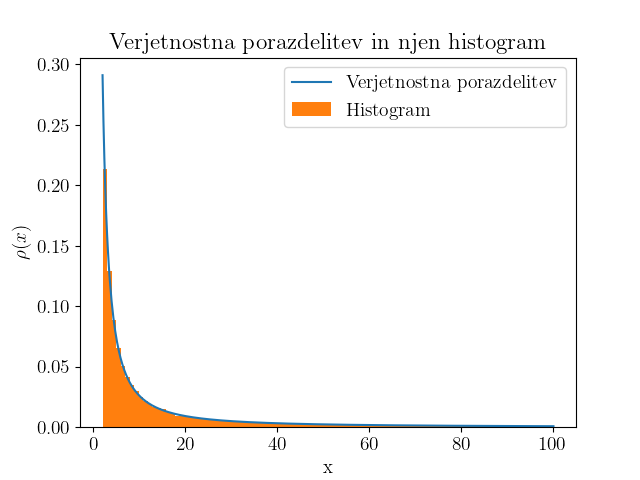
\includegraphics[width=0.7\textwidth]{VerjetnostnaPorazdelitev.png}
    \caption{\label{fig:verjetnost} Graf in histogram verjetnostne porazdelitve med 2 in 100. Začetne vrednost je vzeta za 2, saj naša porazdelitev v izhodišču divergira in sem vzel končno spodno mejo.}
\end{figure}

\subsection*{Polet (Flight)}
Najprej si poglejmo polete, saj so lažji za simuliranje. Za število korakov pri posameznem sprehodu sem vzel $N = \num{10000}$, hkrati pa sem vzporedno simuliral $M = \num{1000}$ poletov. To sem izvedel tako, da sem ustvaril tabelo velikosti $N$x$M$ napolnjeno z naključnimi vrednostmi iz verjetnostne porazdelitve. Najprej sem to tabelo kumulativno seštel po korakih, da sem dobil oddaljenosti po vsakem koraku. Nato sem za vsak korak izračunal MAD (\textit{mean absolute deviation}), kar je neka mera razmazanosti podatkov. V tem primeru je časovna odvisnost kar linearna. Dobljene podatke sem logaritmiral in nanesel na sliko (\ref{fig:flight}). Opazimo dobro prileganje premice. Nato sem enak postopek ponovil za 24 vrednosti $\mu$ med $\num{1.2}$ in $4$, vsakič po $10$x in tako dobil odvisnost $\gamma$ od parametra $\mu$. Opazimo dobro ujemanje s teorijo, kar je prikazano tudi na sliki (\ref{fig:polet}).

\begin{figure}
    \centering
    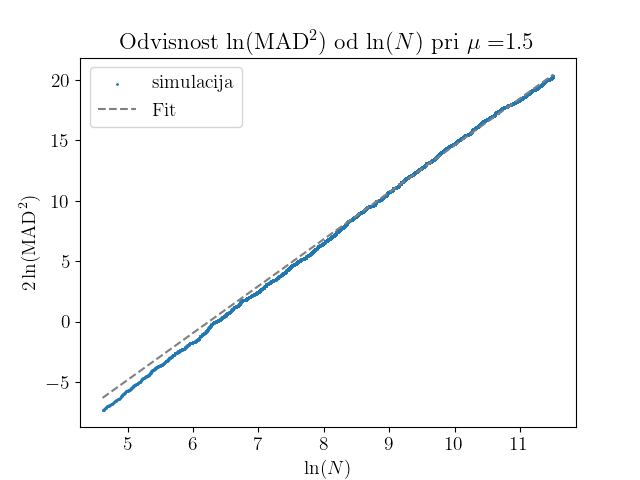
\includegraphics[width=0.7\textwidth]{Flight1_5.png}
    \caption{\label{fig:flight} Graf odvisnosti $2\ln{\mathrm{MAD}}(\ln(N))$, pri parametru $\mu = 1.5$. Pri simulaciji poleta.}
\end{figure}

\begin{figure}
    \centering
    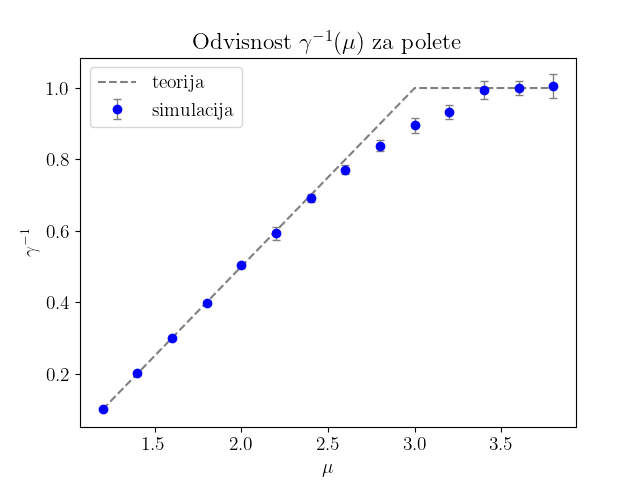
\includegraphics[width=0.7\textwidth]{PoletGammaMu.png}
    \caption{\label{fig:polet} Graf odvisnosti naklona premice od parametra $\mu$. Odstpanje od teoretičnih vrednosti nastopi le pri prehodu med super-difuzivnim in normalno difuzivnim načinom. Pri simulaciji poleta.}
\end{figure}

\subsection*{Sprehod (Walk)}
Tudi v tem načinu je postopek zelo podoben in sem ga z malo razlikami le ponovil. Spremenil sem $M = \num{100}$. Popraviti je bilo tudi potrebno, kako beležim čas, kar sem storil tako, da sem za kumulativno sešteto tabelo izračunal mediano po korakih in jo označil kot nekakšen povprečen čas posameznega koraka. S tem sem potem računal dalje kot prej in dobil graf odvisnosti $2\ln (\mathrm{MAD})$ od $\ln(t)$ na sliki (\ref{fig:walk}). Nato pa tudi odvisnost $\gamma$ od parametra $\mu$. Opazimo dobro, vendar nekoliko slabše kot prej, ujemanje s teorijo, kar je prikazano tudi na sliki (\ref{fig:sprehod}).

\begin{figure}
    \centering
    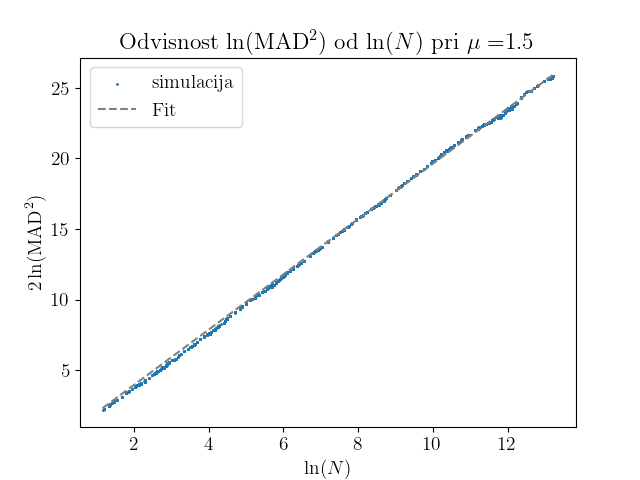
\includegraphics[width=0.7\textwidth]{Walk1_5.png}
    \caption{\label{fig:walk} Graf odvisnosti $2\ln{\mathrm{MAD}}(\ln(t))$, pri parametru $\mu = 1.5$. Pri simulaciji sprehoda.}
\end{figure}

\begin{figure}
    \centering
    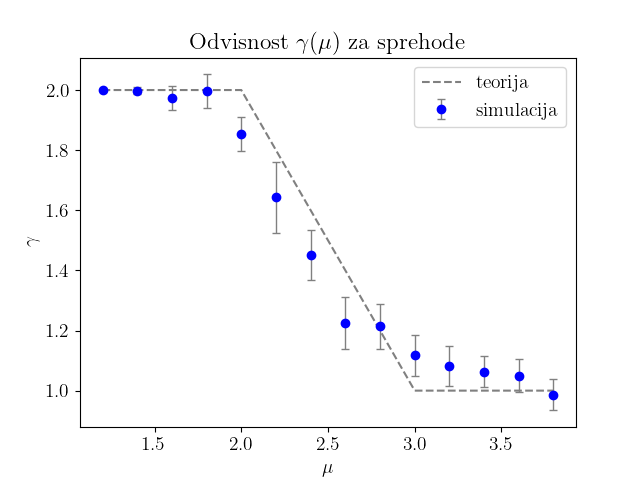
\includegraphics[width=0.7\textwidth]{SprehodGammaMu.png}
    \caption{\label{fig:sprehod} Graf odvisnosti naklona premice od parametra $\mu$. Največje odstopranje je v super-difuzivnem režimu. Pri simulaciji sprehoda.}
\end{figure}

Na koncu sem izrisal nekaj sprehodov različnih dolžin na sliki (\ref{fig:random}).

\begin{figure}
    \centering
    \begin{subfigure}{0.49\textwidth}
        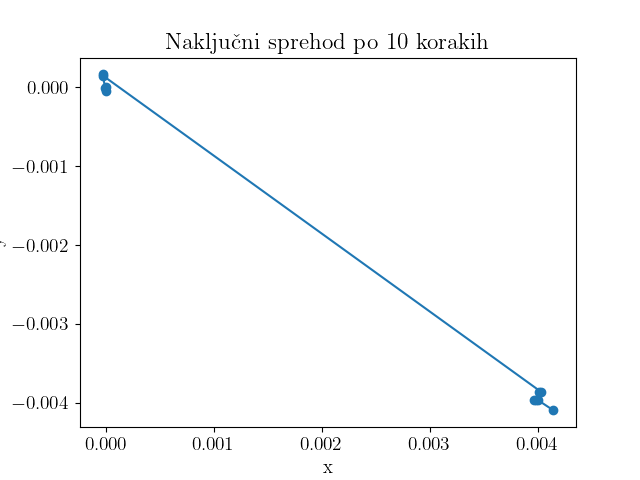
\includegraphics[width=\textwidth]{Random10.png}
    \end{subfigure}
    \begin{subfigure}{0.49\textwidth}
        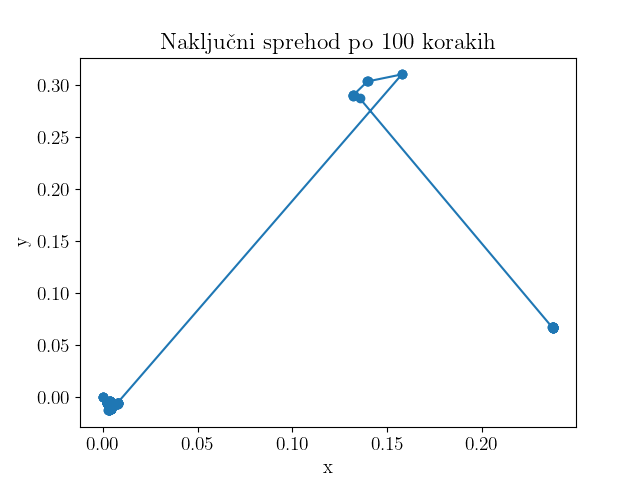
\includegraphics[width=\textwidth]{Random100.png}
    \end{subfigure}
    \begin{subfigure}{0.49\textwidth}
        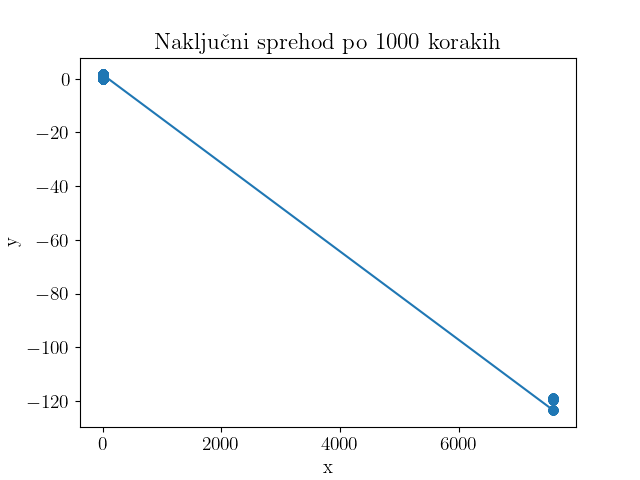
\includegraphics[width=\textwidth]{Random1000.png}
    \end{subfigure}
    \begin{subfigure}{0.49\textwidth}
        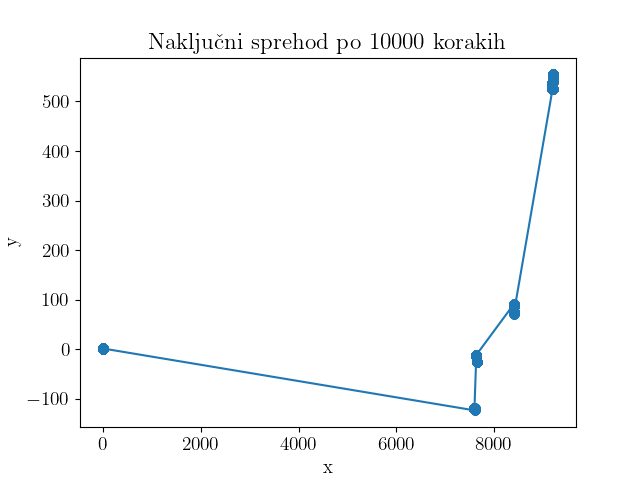
\includegraphics[width=\textwidth]{Random10000.png}
    \end{subfigure}
    \caption{\label{fig:random} Slike štirih različnih dolžin naključnih sprehodov, ki so vsi iz istega semena, torej vsaka naslednja slika vključuje vse prejšnje.}
\end{figure}

\newpage
\section*{Zaključek}
Po zelo veliko časa trajajoči prejšnji nalogi, sem za to sklenil, da jo želim dokončati veliko hitreje. Zadal sem si optimističen cilj $\SI{5}{\hour}$, kar je veliko manj od $\SI{12}{\hour}$, ki sem jih namenil prvi nalogi. Čeprav mi cilja ni uspelo doseči, sta mi izračun in simulacija pri tej nalogi uspeli zelo dobro. Iz stališča kode, mi je uspelo dokončati simulacije z dobrimi rezultati v nekaj več ko $\SI{4}{\hour}$. Z dodatno dobro uro pisanja tega poročila in debati o sami nalogi, bi ocenil čas svojega dela druge naloge na okoli $\SI{6}{\hour}$, kar mislim, da je veliko bolj vzdržno na daljši rok kot prvi teden. To nalogo sem zaradi drugih obveznosti začel reševati šele v torek, samo poročilo pa dokončujem v noči iz srede na četrtek.

% \renewcommand{\bibname}{Literatura}
\begin{thebibliography}{9}

    \bibitem{stackoverflow}
    \url{https://stackoverflow.com/questions/3510475/generate-random-numbers-according-to-distributions}. \\
    Dostopano: 2024-10-17.

\end{thebibliography}

\end{document}